\documentclass[12pt]{article}
\usepackage{graphicx}
\usepackage{fullpage}

\def\sa{\texttt{selectAll(\textless element\textgreater)}}
\def\data{\texttt{data(\textless input data\textgreater)}}
\def\app{\texttt{append(\textless element\textgreater)}}
\def\ent{\texttt{enter()}}

\begin{document}
\title{Data-Vis Assignment 1}
\author{Jack Cassidy \\ Student Number: 1432 0816}
\date{\today}
\maketitle
\section{Basic Shapes}
\begin{figure}[h]
	\centering
	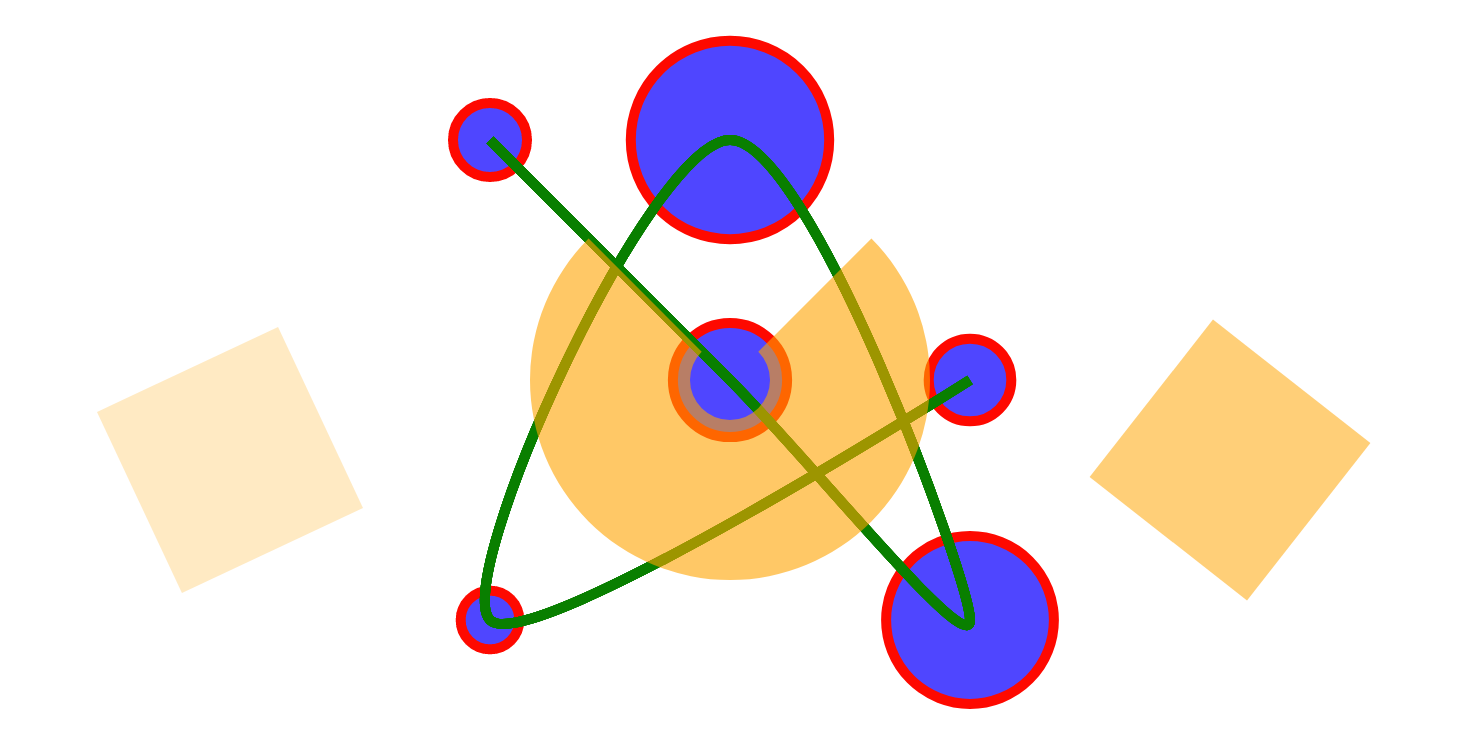
\includegraphics[scale=0.25]{./res/basicshapes}
	\caption{An example of some basic shapes drawn using D3: Circles, Lines \& Curves (Paths) and Arcs.}
	\label{fig:basicshapes}
\end{figure}
\newpage

\section{Minard's Map}
\begin{figure}[h]
	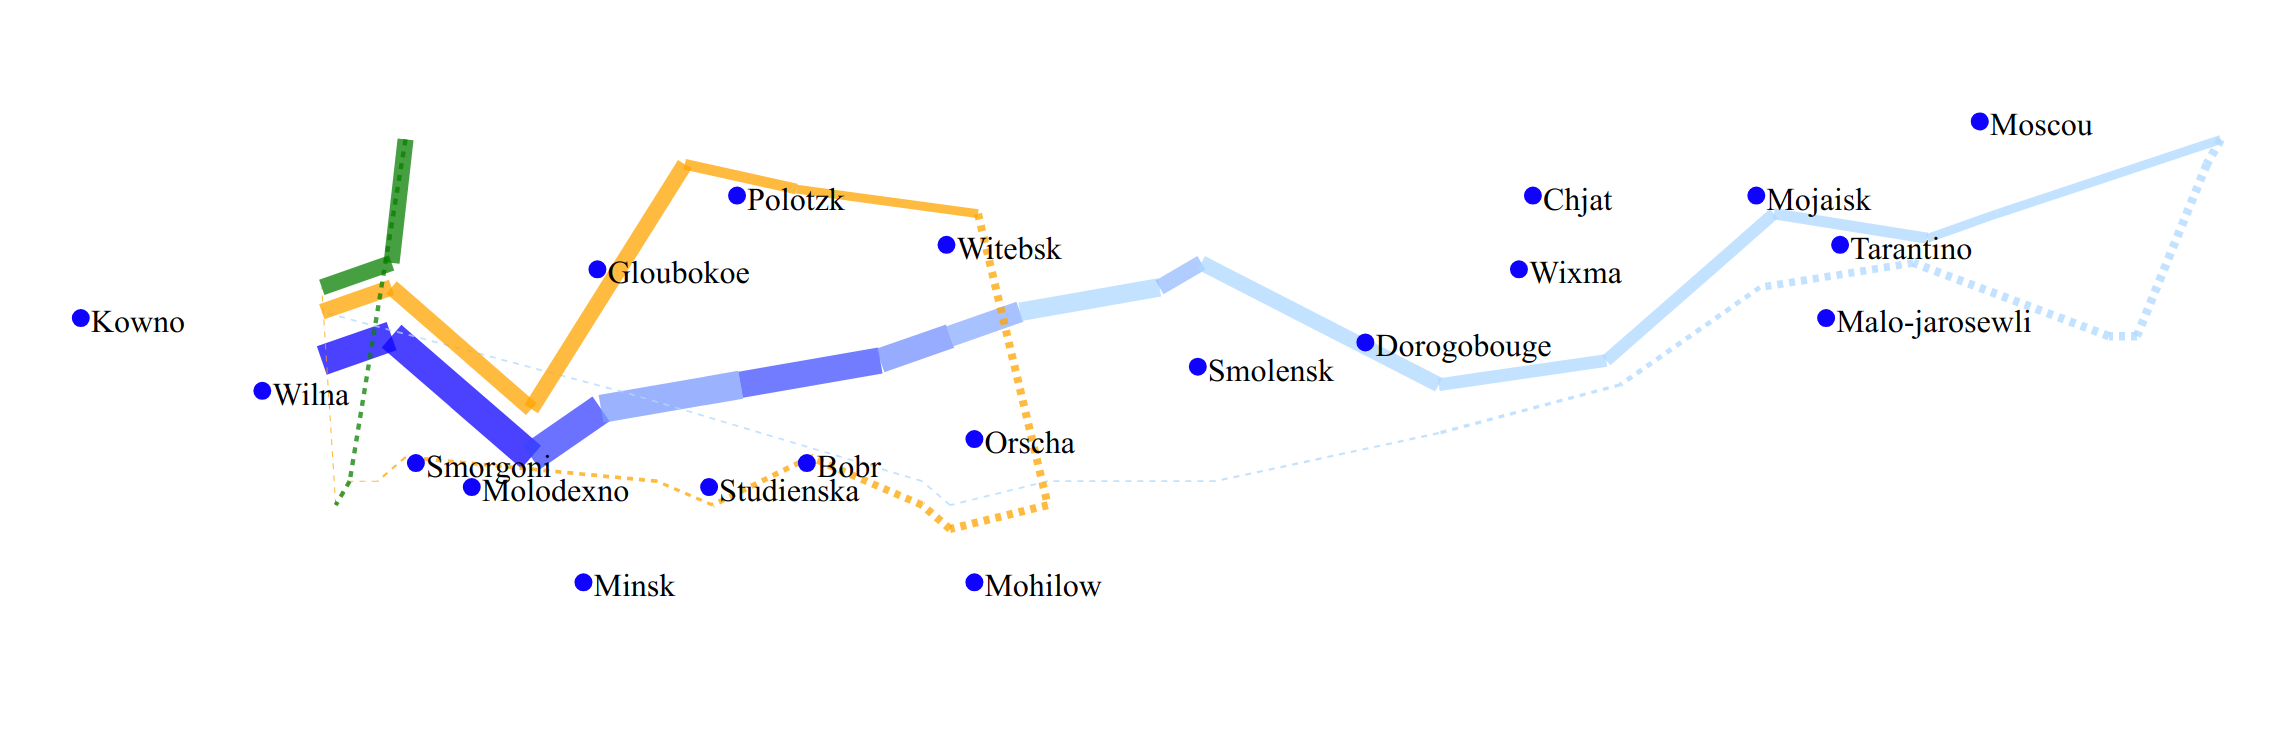
\includegraphics[scale=0.23]{./res/minard}
	\caption{Minard's Map.}
	\label{fig:minard}
\end{figure}

\section{Discussion}
The D3.js Javascript library was used to create the preceding visualizations. Although the learning curve is steep, the rewards are tangible. The general formula for both
images was to create a 1600x500px. SVG and append elements to it using D3 in the \texttt{selectAll(\textless element\textgreater), data(\textless input data\textgreater),
enter(), append(\textless element\textgreater)} pattern.  

This is a widely used pattern, whereby \sa  selects all of the specified elements currently in the DOM (N.B. there may be \textit{none} of these elements currently
present). \data supplies data to the elements in the DOM and any leftover data will be used to create new elements
using \ent and \app.
\subsection{Basic Shapes Discussion}
The circles displayed in Figure~\ref{fig:basicshapes} have centres initialized from a hardcoded array of $cx, cy$ corordinates. The radii and opacity are randomly generated using
\texttt{Math.random()}. The outer red border is created using the \texttt{stroke} attribute and the opacity using the \texttt{fill-opacity} attribute. Each circle is
finally given a fixed translation of 500px, 100px from the $(0, 0)$ origin. 

The curves are created using the \texttt{path} element. A line generator is used to translate circle centres to a path format string, example given below.
\begin{center}
    \texttt{'M 40 40 C 40 40 120 120 160 160 C 200 200 280 300 280 280 C 280 260 200 40 160 40 C 120 40 20 260 40 280 C 60 300 280 160 280 160'}
\end{center}

The curvature is a D3 Cardinal Curve which interpolates the linear path. Finally it is given the same translation as the circles so the path lines up with the centres.  

The arc is very similar to the curves in that it is also a \texttt{path} element, however it has the \texttt{innerRadius, outterRadius, startAngle and endAngle}
attributes to form the arc shape. Here we can see one of the benefits of D3, the ease at which we can do things once the ecosystem is understood.  

Finally the squares are simple \texttt{rect} elements with a random rotation transformation and translated to be equidistant from the central circle.
\subsection{Minard's Map Discussion}
For my visualization of Charles Minard's map, the line colors Blue, Orange and Green represent the 3 Army Divisions. To represent the two stages of the journey, outward
and the return, hatched lines are used for the return portion of each division's trip. The line size decreases with the number of survivors. The decreasing color gradient
as Division 1 (Blue) moves towards Moscow represents the decreasing temperature. Each city is also plotted with a name tag. The lines were generated by converting the
excel data to GeoJSON, which then converts the Longitude and Latitude co-ordinates to a pixel format using a user defined projection. The shapes were generated similarly
to the previous section. Below is some example GeoJSON.
\begin{center}
    \texttt{\{ "type": "Point", "coordinates": [ -105.01621, 39.57422 ] \}}
\end{center}
\end{document}
